Resumidamente o algoritmo denominado \ac{WBAS} estima a frequência $\Omega_m$ por meio da redução do espaço de busca como em uma busca binária tradicional. Nesse contexto, a área do espectro é utilizada como critério de decisão. O exemplo a seguir descreve o algoritmo com mais detalhes.

\subsection{Funcionamento do algoritmo}

Tome $x:\mathbb{Z}\to\mathbb{R}$ da forma
\begin{align*}
    x[n] = \cos(\omega n + \phi), \omega \in [-\pi,\pi]
\end{align*}
Note que, para essa entrada a extração analítica da frequência $\Omega_m$, conforme definido em \ref{sub:model}, é trivial: $\Omega_m = \omega$. 

Considere o filtro complexo ideal $h$ e os filtros reais ideais $a,b$ com respostas em frequência $H,A,B$ descritas abaixo, e na figura \ref{fig:h_a_b}:

\begin{align*}
    H(\Omega) &\triangleq
    \begin{cases}
        1 \text{ se } 0 \leq \Omega \\
        0 \text{ cc }
    \end{cases}\\
    A(\Omega) &\triangleq
    \begin{cases}
        1 \text{ se } \pi/2 \leq \lvert\Omega\rvert \leq \pi\\
        0 \text{ cc }
    \end{cases}\\
    B(\Omega) &\triangleq
    \begin{cases}
        1 \text{ se } 0 \leq \lvert \Omega \rvert < \pi/2\\
        0 \text{ cc }
    \end{cases}
\end{align*}

\begin{figure}[htb]
    \centering
    \caption{Respostas em frequência dos filtros $H$, $A$ e $B$}
    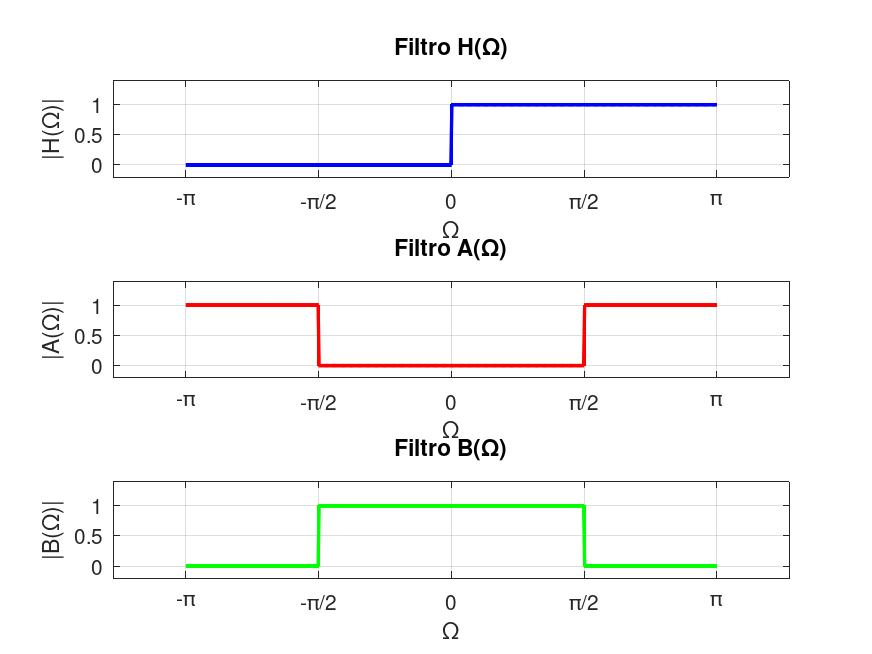
\includegraphics[width=0.8\textwidth]{images/h_a_b.png}
    \label{fig:h_a_b}
    \par\footnotesize Fonte: O autor
\end{figure}

Tome a convolução $x*h$. Como $x$ é real seu espectro possuí simetria conjugada, assim o resultado da operação é a remoção da componente simétrica negativa como na imagem \ref{fig:x+}. A partir desse passo ignoram-se as frequências negativas durante as demonstrações e gráficos.

\begin{align*}
    X^+\triangleq X(\Omega)\times H(\Omega) =
    \begin{cases}
        X(\Omega) \text{ se } 0 \leq \Omega \\
        0 \text{ cc }
    \end{cases}
\end{align*}

\begin{figure}[htb]
    \centering
    \caption{Remoção de frequências negativas}
    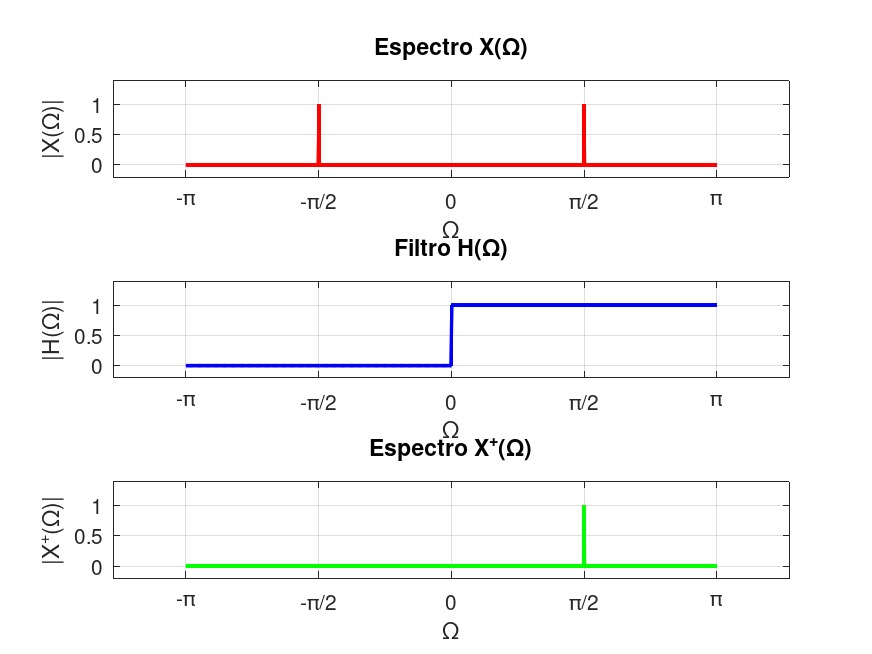
\includegraphics[width=0.8\textwidth]{images/x+.png}
    \label{fig:x+}
    \par\footnotesize Fonte: O autor
\end{figure}

Em seguida, é feita a aplicação de $a,b$ sobre o sinal resultante. Nessa etapa ocorre a decomposição em uma banda de alta frequência e uma de baixa.

\begin{align*}
    X_a(\Omega) \triangleq X^+(\Omega)\times A(\Omega) =
    \begin{cases}
        X(\Omega) \text{ se } \pi/2 \leq \Omega \leq \pi\\
        0 \text{ cc }
    \end{cases}\\
    X_b(\Omega) \triangleq X^+(\Omega)\times B(\Omega) =
    \begin{cases}
        X(\Omega) \text{ se } 0 \leq \Omega < \pi/2\\
        0 \text{ cc }
    \end{cases}\\
\end{align*}

Pelo teorema de Parseval \eqref{eq:Parseval}, a energia contida no espectro do sinal é idêntica à contida no domínio do tempo (salvo uma constante de normalização). Dessa forma é determinada a energia contida nas altas ($E_a$) e baixas ($E_b$) frequências, por meio dos sinais $x_a$ e $x_b$.

\begin{align*}
    E_a = \sum_{n=0}^{N-1}\lvert x_a[n] \rvert^2 = \int_{-\pi}^{\pi}\lvert X_a(\Omega) \rvert^2 d\Omega\\
    E_b = \sum_{n=0}^{N-1}\lvert x_b[n] \rvert^2 = \int_{-\pi}^{\pi}\lvert X_b(\Omega) \rvert^2 d\Omega\\
\end{align*}

Os valores $E_a, E_b$ podem ser utilizados como métricas de decisão da busca binária, conforme o lema e corolário a seguir mostram, bem como a imagem \ref{fig:ea_eb}:

\vspace{1cm}
\begin{lemma}
\label{lma:criterea}
Seja $\Omega_m \in [0,\pi]$ então: $\Omega_m \in [0,\pi/2) \iff E_a < E_b$
\begin{proof}

    \medskip
    \textbf{Ida:} $\Omega_m \in [0,\pi/2) \implies E_a < E_b$
    \begin{align*}
        E_a &= \int_{\pi/2}^{\pi} \lvert X(\Omega) \rvert^2 = \int_{\pi/2}^{\pi}  \delta(\Omega-\Omega_m) = 0\\
        E_b &= \int_{0}^{\pi/2} \lvert X(\Omega) \rvert^2 = \int_{0}^{\pi/2} \delta(\Omega-\Omega_m) = 1\\
        &\therefore \Omega_m \in [0,\pi/2) \implies E_a < E_b
    \end{align*}
    
    \medskip
    \textbf{Volta:} $E_a < E_b \implies \Omega_m \in [0,\pi/2)$

    Suponha por contradição que $\Omega_m \in [\pi/2,\pi]$, então:
    \begin{align*}
        &\int_{\pi/2}^{\pi} \delta(\Omega-\Omega_m) < \int_{0}^{\pi/2} \delta(\Omega-\Omega_m) \iff 1 < 0\\
        &\text{contradição!} \therefore \Omega_m \notin [\pi/2,\pi]\\
        &\Omega_m \in [0,\pi] \setminus [\pi/2,\pi] \implies \Omega_m \in [0,\pi/2)
    \end{align*}
\end{proof}
\end{lemma}

\begin{clry}
\label{clry:complementary}
$\Omega_m \in [\pi/2,\pi] \iff E_b \leq E_a$
\begin{proof}
    Tomando a negação do Lema~\ref{lma:criterea}:
    \begin{align*}
        \Omega_m \notin [0,\pi/2) &\iff \neg(E_a < E_b)\\
        \Omega_m \in [0,\pi] \setminus [0,\pi/2) &\iff E_b \leq E_a\\
        \Omega_m \in [\pi/2,\pi] &\iff E_b \leq E_a
    \end{align*}
\end{proof}
\end{clry}

\begin{figure}[htb]
    \centering
    \caption{Decisão entre as bandas $E_a$, $E_b$}
    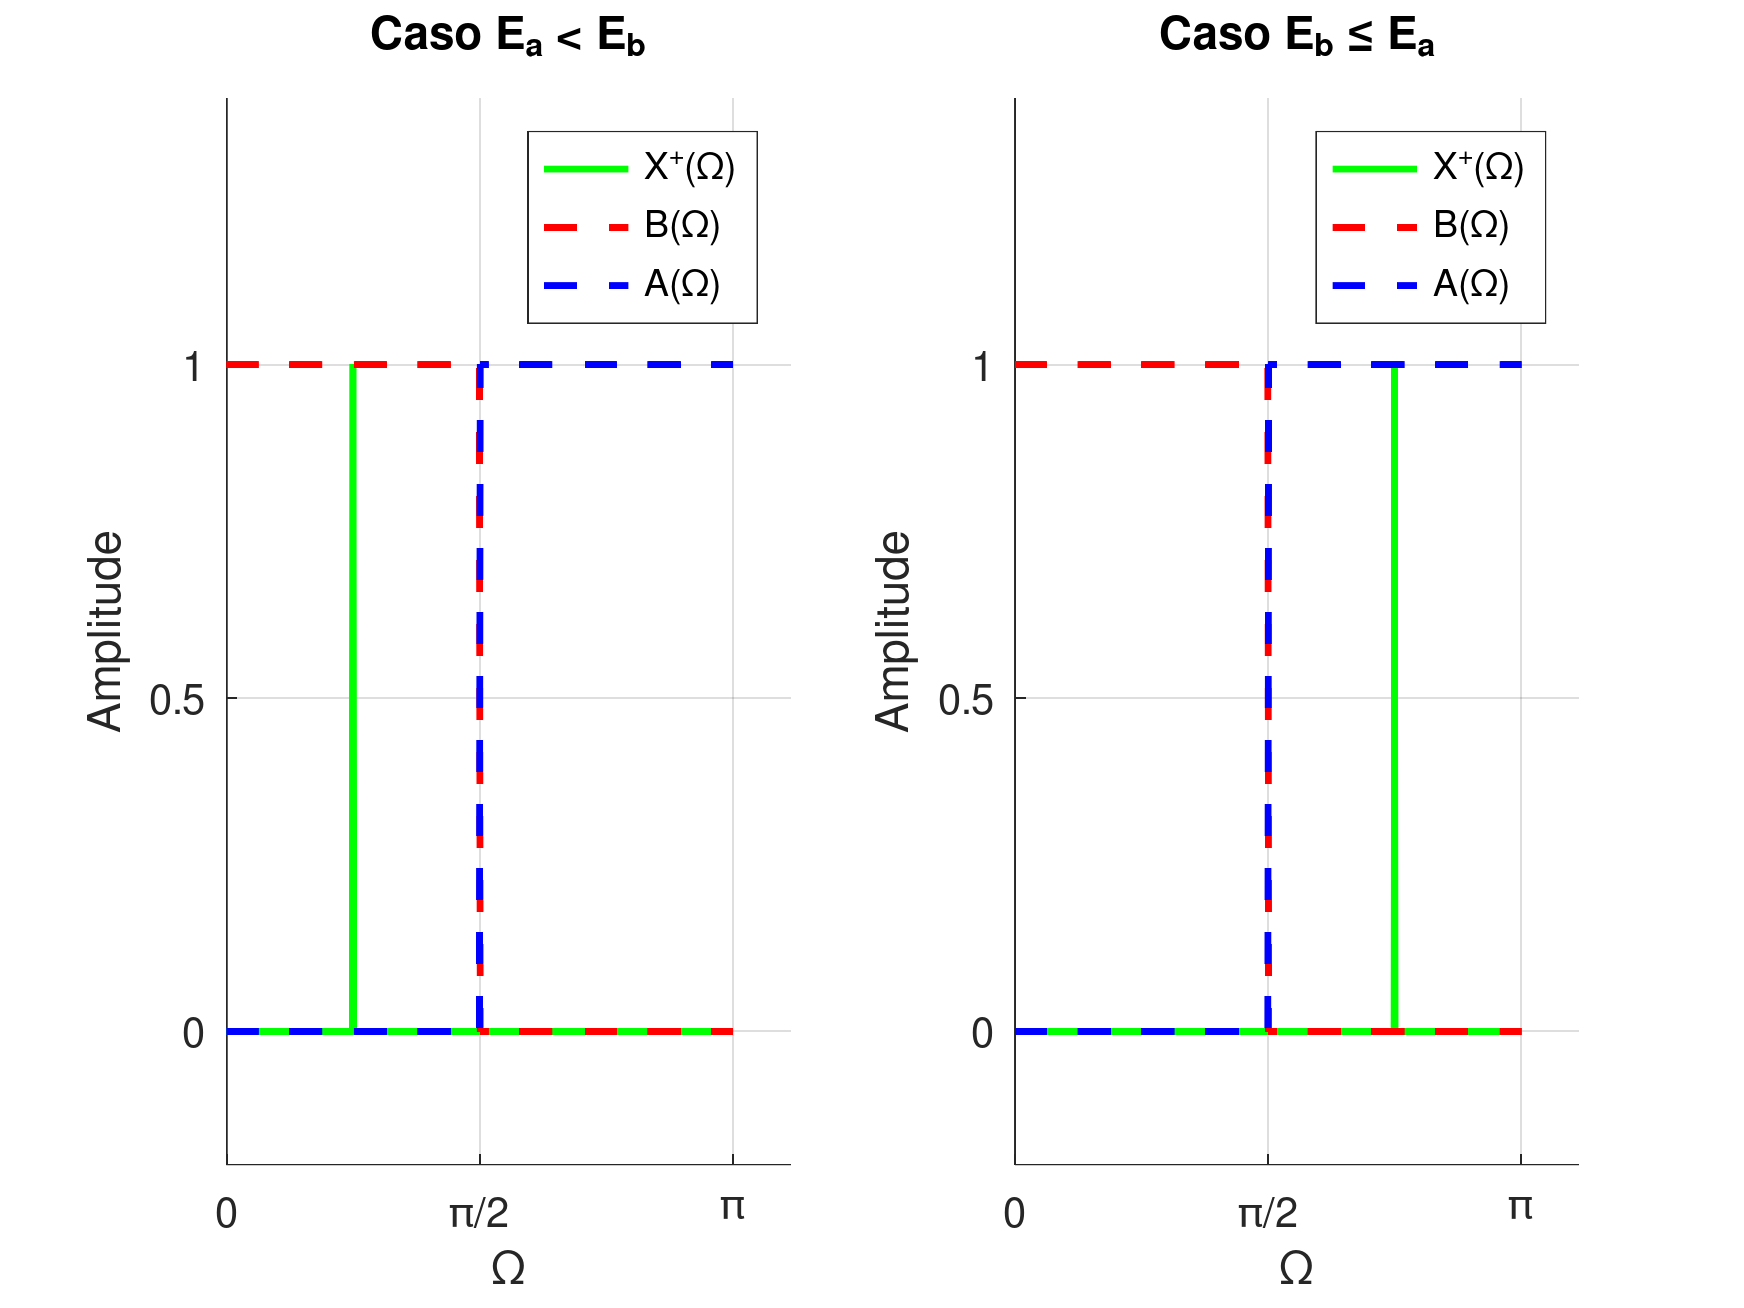
\includegraphics[width=0.8\textwidth]{images/ea_eb.png}
    \label{fig:ea_eb}
    \par\footnotesize Fonte: O autor
\end{figure}

Em ambos os casos, faz-se uma decisão gulosa entre a energia em uma das bandas, de forma que o espaço de busca é reduzido pela metade.

Pelo teorema de Nyquist \ref{eq:Nyquist}, para uma representação sem \textit{aliasing}, a frequência de amostragem do sinal deve ser o dobro de sua frequência máxima. No caso em que $E_a < E_b$, o sinal de interesse passa a ser limitado à banda $[0,\pi/2]$, sua frequência máxima é reduzida pela metade, permitindo a decimação sem \textit{aliasing}.

Mesmo que $E_b \leq E_a$ ainda é possível decimar metade das amostras. Basta transladar o intervalo de frequências de $[\pi/2,\pi]$ para $[0,\pi/2]$ por meio de uma multiplicação por uma exponencial complexa. Com isso a frequência máxima é novamente reduzida, e o sinal pode ser decimado.

Esse mesmo procedimento pode ser repetido recursivamente: filtra-se a entrada com $a,b$, determina-se a energia de $E_a,E_b$ pela aplicação de Parseval em $x_a,x_b$, decide-se pela maior energia e decima-se o sinal, possivelmente realizando uma multiplicação complexa antes. O algoritmo para quando o sinal não pode mais ser decimado.

A cada iteração o espaço de busca, bem como a dimensão da entrada são divididos pela metade. A estimativa de $\Omega_m$ é codificada na sequência de escolhas entre $E_a,E_b$. Caso se escolha por $E_a$ o espaço de busca $[b,a]$ deve tornar-se $[\frac{b+a}{2},a]$, caso contrário $[b,\frac{b+a}{2}]$, analogamente, no primeiro caso decima-se (e multiplica-se) $x_a$ e no segundo $x_b$.

As decimações e multiplicações alteram a frequência efetiva observada por cada iteração do algoritmo. Por exemplo, na primeira iteração $\Omega_m^0$, a frequência observada é idêntica à $\Omega_m$, na segunda a depender se o sinal foi decimado, ou decimado e multiplicado observa-se $\Omega_m^1 = 2\Omega_m$ ou $\Omega_m^1 = 2\Omega_m-\pi$ respectivamente. Em geral, tem-se o lema:

\vspace{1cm}
\begin{lemma}
\label{lma:update}
Seja $k$ o número da iteração, define-se $\Omega_m^k$ como a frequência do sinal na iteração $k$. Sejam $x^k$, $x_a^k$ e $x_b^k$ respectivamente: sinal na iteração $k$, o sinal na iteração $k$ filtrado por $a$ e o sinal na iteração $k$ filtrado por $b$. Sejam $E_a^k$ e $E_b^k$ as energias associadas à $x_a^k$ e $x_b^k$. Então:

\begin{align*}
    \Omega_m^{k+1} =
    \begin{cases}
        2\Omega_m^k \text{ se } E_a^k < E_b^k\\
        2\Omega_m^k - \pi \text{ se } E_b^k \leq E_a^k
    \end{cases}
\end{align*}
\begin{proof}

    \medskip
    \textbf{Caso $E_a^k < E_b^k$:}
    \begin{align*}
        &E_a^k < E_b^k \implies x^{k+1} = \downarrow_2 x_b^k\\
        &x^{k+1}[n] = x_b^k[2n] = e^{j\Omega_m^k (2n)} = e^{j(2\Omega_m^k)n}\\
        &\therefore \Omega_m^{k+1} = 2\Omega_m^k
    \end{align*}

    \medskip
    \textbf{Caso $E_b^k \leq E_a^k$:}
    \begin{align*}
        &E_b^k \leq E_a^k \implies x^{k+1} = \downarrow_2 (x_a^k \cdot e^{-j\pi n/2})\\
        &x^{k+1}[n] = x_a^k[2n] \cdot e^{-j\pi n} = e^{j\Omega_m^k(2n)} \cdot e^{-j\pi n} = e^{j(2\Omega_m^k - \pi)n}\\
        &\therefore \Omega_m^{k+1} = 2\Omega_m^k - \pi
    \end{align*}
\end{proof}
\end{lemma}

O lema a seguir deixa clara a relação entre $\Omega_m$ e $\Omega_m^k$:

\vspace{1cm}
\begin{lemma}
\label{lma:mapping}
Com as definições de \ref{lma:update}, e tomando $b_0 = 0$, $a_0 = \pi$ e
$\Omega_m^0 = \Omega_m$, então $\Omega_m^k$ mapeia linearmente
$\Omega_m \in [b_k, a_k]$ para $[0,\pi]$:
\begin{align*}
    \Omega_m = \frac{a_k - b_k}{\pi}\Omega_m^k + b_k
\end{align*}
\begin{proof}

    \textbf{Caso Base ($k=0$):}
    \begin{align*}
        \Omega_m^0 = \Omega_m,\quad b_0 = 0,\quad a_0 = \pi\\
        \frac{a_0 - b_0}{\pi}\Omega_m^0 + b_0 = \frac{\pi}{\pi}\Omega_m + 0 = \Omega_m \quad\checkmark
    \end{align*}
    
    \textbf{Hipótese Indutiva:} Suponha que para $k$ vale:
    $$\frac{a_k-b_k}{\pi}\Omega_m^k + b_k = \Omega_m$$

    \textbf{Passo Indutivo:}
    
    \medskip
    \textbf{Caso $\Omega_m^k \in [0,\pi/2)$:} Conforme \ref{lma:criterea}, $\Omega_m^k \in [0,\pi/2) \iff E_a^k < E_b^k$. Então os valores serão atualizados assumindo a banda inferior conforme \ref{lma:update}, em particular:
    
    \begin{align*}
        &\Omega_m^{k+1} = 2\Omega_m^k \therefore \Omega_m^{k+1} \in [0,\pi)\\
        &a_{k+1} = \frac{a_k+b_k}{2},\quad b_{k+1}=b_k\\
    \end{align*}

    Verificando a hipótese indutiva:

    \begin{align*}
        \frac{a_{k+1}-b_{k+1}}{\pi}\Omega_m^{k+1}+b_{k+1}
        &= \frac{\frac{a_k+b_k}{2}-b_{k}}{\pi}\cdot 2\Omega_m^{k}+b_{k}\\ 
        &= \frac{a_k-b_{k}}{\pi}\Omega_m^{k}+b_{k} = \Omega_m \quad\checkmark
    \end{align*}

    \medskip
    \textbf{Caso $\Omega_m^k \in [\pi/2,\pi]$:} Conforme \ref{clry:complementary}, $\Omega_m^k \in [\pi/2,\pi] \iff E_b^k \leq E_a^k$. Então os valores serão atualizados assumindo a banda superior conforme \ref{lma:update}, em particular:

    \begin{align*}
        &\Omega_m^{k+1} = 2\Omega_m^k - \pi \therefore \Omega_m^{k+1} \in [0,\pi)\\
        &b_{k+1} = \frac{a_k+b_k}{2},\quad a_{k+1}=a_k\\
    \end{align*}

    Verificando a hipótese indutiva:

    \begin{align*}
        \frac{a_{k+1}-b_{k+1}}{\pi}\Omega_m^{k+1}+b_{k+1}
        &= \frac{a_k-\frac{a_k+b_k}{2}}{\pi}(2\Omega_m^{k}-\pi)+\frac{a_k+b_k}{2}\\ 
        &= \frac{a_k-b_{k}}{\pi}\Omega_m^{k}+b_k = \Omega_m \quad\checkmark
    \end{align*}
    
\end{proof}
\end{lemma}

\subsection{Convergência para tons puros assumindo filtros ideais}

A seguir prova-se a convergência para o caso de uso mais simples do algorítimo. Essa análise pode ser expandida para formular um critério de convergência genérico, bem como incluir  o uso de filtros não ideais, mas entende-se que fazê-lo seria fora do escopo desse documento.

\begin{thm}
Tome $x:\mathbb{Z}\to\mathbb{R}$ da forma
\begin{align*}
    x[n] = \cos(\Omega_m n + \phi), \Omega_m \in [-\pi,\pi]
\end{align*}
então \ac{WBAS} converge para $\Omega_m$
\end{thm}

\begin{proof}

\textbf{Caso Base ($k=0$):}
\begin{align*}
    &b_0 = 0,\quad a_0 = \pi\\
    &\Omega_m \in [0,\pi] = [b_0, a_0] \quad\checkmark
\end{align*}

\textbf{Hipótese Indutiva:} Suponha que para $k$:
$$\Omega_m \in [b_k, a_k]$$

\textbf{Passo Indutivo:}

Invertendo o mapeamento em \ref{lma:mapping}:
\begin{align*}
    &\frac{a_k-b_k}{\pi}\Omega_m^k+b_k = \Omega_m\\
    &\Omega_m^k = \frac{\pi}{a_k-b_k}(\Omega_m - b_k)
\end{align*}

\medskip
\textbf{Caso $\Omega_m \in [b_k,\frac{a_k+b_k}{2})$:} Determinando os limites de $\Omega_m^k$ a partir de $\Omega_m$:
\begin{align*}
    \Omega_m^k &\in \left[\frac{\pi}{a_k-b_k}(b_k-b_k),\,\frac{\pi}{a_k-b_k}\left(\frac{a_k+b_k}{2}-b_k\right)\right)\\
    &\in [0,\pi/2) \quad\text{aplica-se o Lema~\ref{lma:criterea}}
\end{align*}

Logo os valores são atualizados assumindo a banda inferior: $a_{k+1} = \frac{b_k+a_k}{2}$,
$b_{k+1} = b_k$, resultando no intervalo $[b_{k+1}, a_{k+1}] = [b_k, \frac{a_k+b_k}{2}]$.
Como $\Omega_m \in [b_k, \frac{a_k+b_k}{2}) \subset [b_{k+1}, a_{k+1}]$,
então $\Omega_m \in [b_{k+1}, a_{k+1}]$ e a hipótese indutiva vale para $k+1$.

\medskip
\textbf{Caso $\Omega_m \in [\frac{a_k+b_k}{2},a_k]$:} Determinando os limites de $\Omega_m^k$ a partir de $\Omega_m$:
\begin{align*}
    \Omega_m^k &\in \left[\frac{\pi}{a_k-b_k}\left(\frac{a_k+b_k}{2}-b_k\right),\,\frac{\pi}{a_k-b_k}(a_k-b_k)\right]\\
    &\in [\pi/2,\pi] \quad\text{aplica-se o Corolário~\ref{clry:complementary}}
\end{align*}

Logo os valores são atualizados assumindo a banda superior: $a_{k+1} = a_k$,
$b_{k+1} = \frac{b_k+a_k}{2}$, resultando no intervalo $[b_{k+1}, a_{k+1}] = [\frac{b_k+a_k}{2}, a_k]$.
Como $\Omega_m \in [\frac{b_k+a_k}{2}, a_k] = [b_{k+1}, a_{k+1}]$,
então $\Omega_m \in [b_{k+1}, a_{k+1}]$ e a hipótese indutiva vale para $k+1$.
\end{proof}

\subsection{Análise assintótica e velocidade de convergência}

Como dito anteriormente, a cada iteração $k$ o tamanho da entrada, bem como o espaço de busca diminuem pela metade. Assim é fácil de verificar que o número de total de iterações é dado por $log_2(n)$, onde $n$ representa a dimensão da entrada. Portanto, o espaço de busca será dividido em duas partes $log_2(n)$ vezes, produzindo uma velocidade de convergência na ordem:

\begin{align*}
O(\frac{1}{2^{log_2(n)}}) = O(1/n)
\end{align*}

A função de custo do algorítimo é dada pela soma do custo de cada uma das $log_2(n)$ iterações. Em uma única iteração são executadas operações de custo linear com a entrada, e cada iteração diminuí o tamanho da entrada na metade, assim:

\begin{align*}
&O(\sum^{log_2{n}-1}_{k=0} \frac{n}{2^k}) =\\
&O(2n - 2) = \\
&O(n)
\end{align*}

A complexidade obtida (linear) corresponde a uma classe assintótica menor em relação ao algorítimo estado da arte \ref{sub:stateoftheart} ($nlog(n)$). Ou seja, existirá algum valor de $n$ para qual o \ac{WBAS} é sempre mais computacionalmente eficiente.

\subsection{Algorítimo predecessor}

O \ac{WBAS} foi desenvolvido com base nos conhecimentos adquiridos com a implementação do \ac{BAS}. A ideia central dos algorítimos é a mesma: busca binária utilizando a área do espectro como critério de decisão, no entanto, o mecanismo utilizado para o cálculo da área diverge.

Enquanto o \ac{WBAS} utiliza filtros e o teorema de Parseval \eqref{eq:Parseval}, o \ac{BAS} utiliza uma aproximação junto ao algorítimo de Goertzel \ref{sub:Goertzel}. A aproximação do \ac{BAS} tenta determinar o valor de \eqref{eq:bastgt}, ...

\begin{align}
    \label{eq:bastgt}
    \int_{\alpha}^{\alpha + \Delta} \lvert X(\Omega) \rvert^{2n} d\Omega
\end{align}

\subsection{Implementação}

\subsubsection{Infraestrutura}

O foco em desempenho na concepção do \ac{WBAS} veio da intenção de torná-lo compatível com processamento em tempo real em sistemas embarcados. Nesse sentido tornou-se necessário uma plataforma de coleta de amostras em tempo real, permitindo testes no ambiente de operação projetado.

Também para propósitos de teste e validação, tornou-se necessário visualizar o espectro das amostras coletadas. Com isso, a convergência pode ser verificada observando o comportamento do algorítimo dado um sinal conhecido.

==dados do proj? (i.e orientador, colaboradores, ...)==. ==Dar crédito para a Fernanda pq vou usar os diagramas dela==.

Essas implementações satélite culminaram em um projeto de iniciação científica, no qual foi desenvolvido um analisador de espectro que monitora a saída de áudio do computador e exibe as magnitudes das frequências selecionadas. A estrutura do projeto é descrita no diagrama \ref{fig:spectrum_analizer}.
            
\begin{figure}[htb]
    \centering
    \caption{Esquemático do analizador}
    \includegraphics[width=0.8\textwidth]{images/spectrum_analizer.png}
    \label{fig:spectrum_analizer}
    \par\footnotesize Fonte: ==Fernanda==
\end{figure}

São dois os componentes de \textit{software} principais desenvolvidos: o \textit{FrontEnd} e o \textit{BackEnd}, ambos implementados em classes \textbf{C++} de mesmo nome. O \textit{FrontEnd} utiliza a biblioteca \textit{DearImGUI} e \textit{DearImPlot} \ref{sub:dear} para exibir as informações obtidas pelo \textit{BackEnd}. Paralelamente, o \textit{BackEnd}, por meio da biblioteca \textit{PulseAudio} \ref{sub:pulseaudio}, grava amostras da fonte de áudio especificada pelo usuário, e extraí o conteúdo em frequência da gravação por meio de instâncias do algorítimo de Goertzel \ref{sub:Goertzel}. 

Arquiteturalmente, o \textit{BackEnd} é a entidade passiva, requisições são feitas do mestre (\textit{FrontEnd}) ao escravo (\textit{BackEnd}) por meio de chamadas de funções. Essa divisão permitiu o desenvolvimento independente dos módulos. 

As imagens \ref{fig:sources}, \ref{fig:magxtime} e \ref{fig:spectogram} exibem as funcionalidades do analisador. Em \ref{fig:sources} é exibida a tela de comando, nessa é possível escolher a fonte de áudio e gerenciar as instâncias do algorítimo de Goertzel. Sendo possível criar instâncias para monitorar uma frequência específica, remover instâncias ou pausá-las.

A imagem \ref{fig:magxtime} mostra um gráfico de magnitude por tempo. Para cada frequência monitorada produz-se esse gráfico, nele são exibidos últimos duzentos valores de magnitude mais recentes.

Finalmente a figura \ref{fig:spectogram} mostra o gráfico de espectrograma. Esse consolida as informações de todos os analisadores ativos: o eixo da abscissa corresponde ao índice das duzentas amostras mais recentes, o eixo das ordenadas corresponde a cada uma das frequências monitoradas, para cada par frequência x índice é associada uma cor que corresponde à intensidade daquela frequência naquele índice.

\begin{figure}[htb]
    \centering
    \caption{Tela de Configuração do Analizador}
    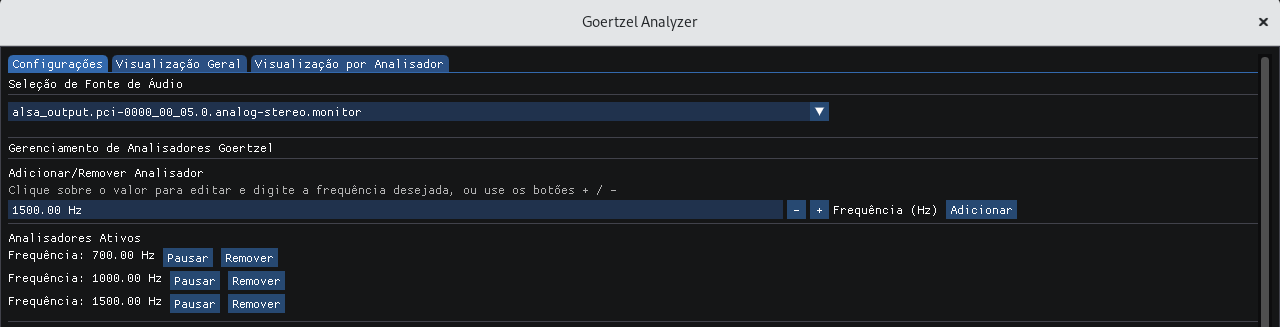
\includegraphics[width=0.8\textwidth]{images/sources.png}
    \label{fig:sources}
    \par\footnotesize Fonte: ==Fernanda==
\end{figure}

\begin{figure}[htb]
    \centering
    \caption{Magnitude x Tempo}
    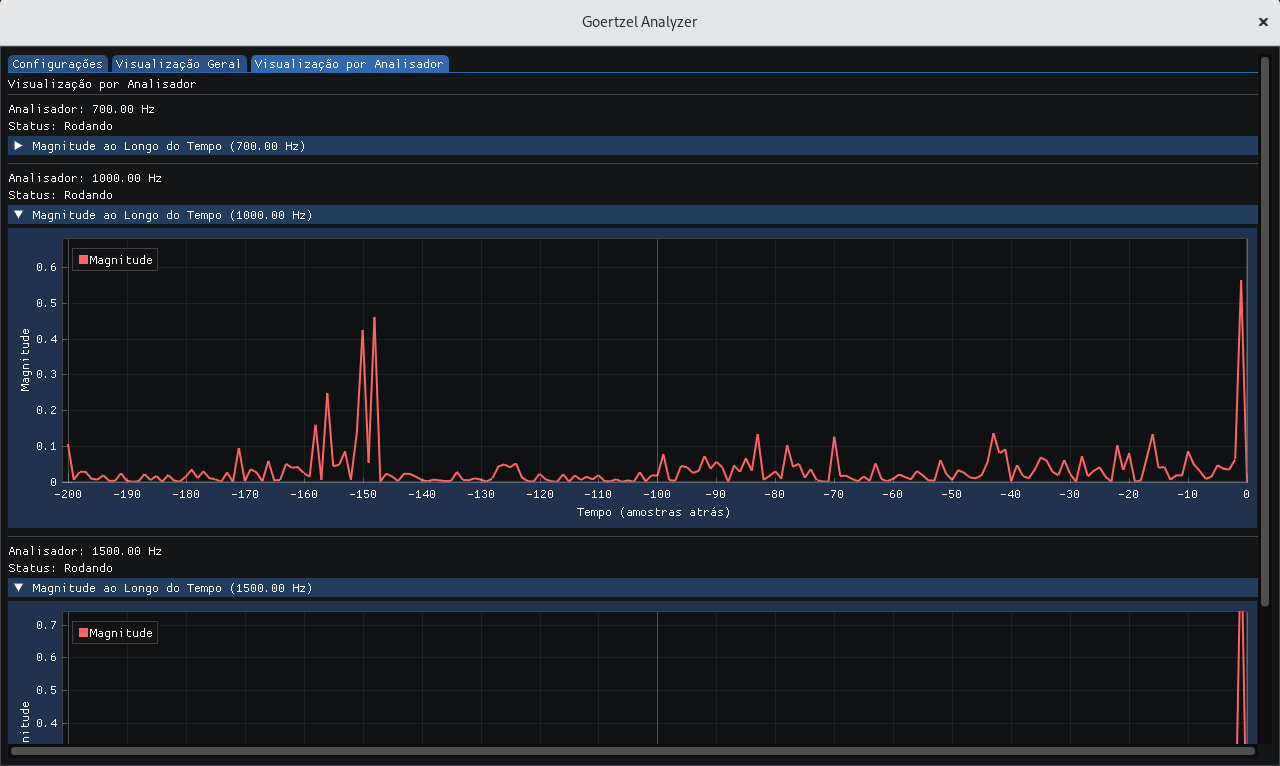
\includegraphics[width=0.8\textwidth]{images/magxtime.png}
    \label{fig:magxtime}
    \par\footnotesize Fonte: ==Fernanda==
\end{figure}

\begin{figure}[htb]
    \centering
    \caption{Espectrograma}
    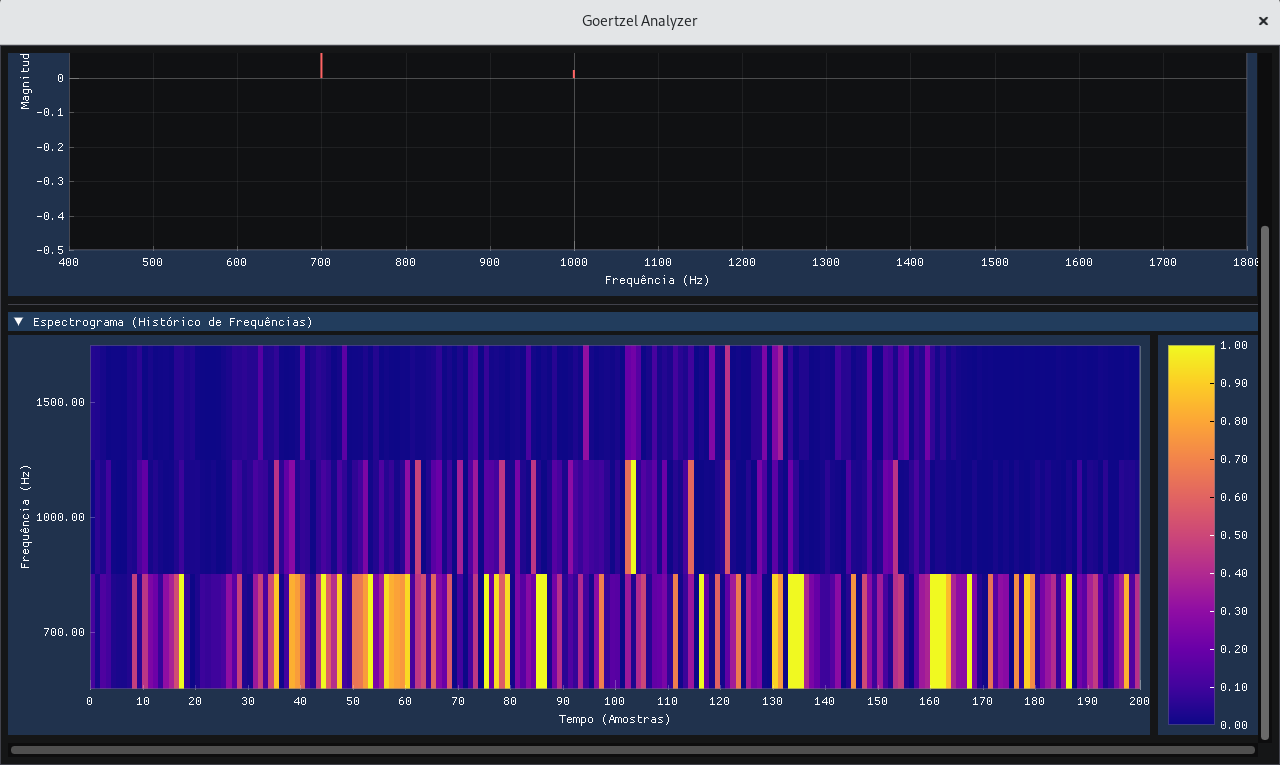
\includegraphics[width=0.8\textwidth]{images/spectogram.png}
    \label{fig:spectogram}
    \par\footnotesize Fonte: ==Fernanda==
\end{figure}



\subsubsection{Algorítimo}